\section{Архитектура}

Как упоминалось выше, приложение собирается при помощи фреймворка Maven, поэтому было принято решение естественным
образом разделить приложение на несколько логических единиц "--- модулей Maven. Схема зависимостей между модулями
приложения приведена на рис.~\ref{architecture}.

\begin{figure}[h]
\center{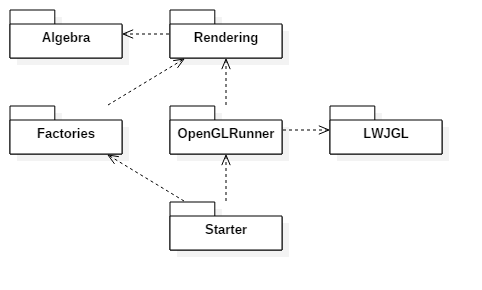
\includegraphics[scale=0.8]{architecture}}
\caption{Архитектура приложения}
\label{architecture}
\end{figure}

Таким образом, приложение состоит из пяти модулей:

\begin{itemize}

\item \texttt{Algebra} "--- модуль алгебраических объектов, содержит классы основных алгебраических объектов,
используемых в приложении (векторы, матрицы, кватернионы, функции и~т.~п.), а также алгоритмические решения некоторых
простейших алгебраических задач;
\item \texttt{Rendering} "--- модуль рендеринга, содержит основную логику графического движка, не завязанную
на конкретную реализацию отрисовки на экране;
\item \texttt{Factories} "--- модуль алгоритмов, содержит классы-фабрики, создающие массивы 3D-объектов и анимаций для
отрисовки на экране, а также "--- реализованные алгоритмы построения сплайн-кривых;
\item \texttt{OpenGLRunner} "--- модуль интеграции с OpenGL, содержит реализацию рендеринга посредством библиотеки
LWJGL, а также основной код для запуска приложения с использованием данной библиотеки.
\item \texttt{Starter} "--- модуль запуска приложения, содержит единственный класс \texttt{Main}, запускающий
приложение с реализацией рендеринга из модуля \texttt{OpenGLRunner} и с несколькими классами-фабриками из модуля
\texttt{Factories}.
\end{itemize}

В последующих разделах следует подробное описание самых объёмных модулей реализованного приложения.
